\documentclass[xcolor={usenames,dvipsnames,svgnames,table}]{beamer}

\mode<presentation>
\usetheme{Madrid}

\usecolortheme[RGB={80,0,0}]{structure}
\useoutertheme[subsection=false]{miniframes}
\useinnertheme{default}

% hide navigation controlls
\setbeamertemplate{navigation symbols}{}

\setbeamercolor{normal text}{fg=black}
\setbeamercovered{dynamic}
\beamertemplatetransparentcovereddynamicmedium
%\usepackage{chronology}
\setbeamertemplate{caption}[numbered]

\definecolor{Maroon}{RGB}{80,0,0}
\definecolor{BurntOrange}{RGB}{204,85,0}


% load macros and prevent authblk from loading
\makeatletter
% prevent a package from loading
\newcommand{\dontusepackage}[2][]{%
    \@namedef{ver@#2.sty}{9999/12/31}%
    \@namedef{opt@#2.sty}{#1}
}

% a macro to load packages only if they are not yet loaded, needed for combination of beamer and hyperref
\newcommand{\usepackagesave}[2][{}]{
    \ltx@ifpackageloaded{#2}{}{
        \usepackage[#1]{#2}}
}
\makeatother
\dontusepackage{authblk}

% load packages, settings and definitions
% this file contains all commonly used packages for the Rattlesnake documentation
% new package, add comment what they are used for

% command packages
\usepackage{xifthen}     % if -then else command

% language and font improvements
\usepackage[english]{babel}	% Multilingual support - https://www.ctan.org/pkg/babel
\usepackage[utf8]{inputenc} % Accept different input encodings - https://www.ctan.org/pkg/inputenc
\usepackage[kerning,spacing,babel]{microtype} % Subliminal refinements towards typographical perfection - https://www.ctan.org/pkg/microtype
\usepackage{eepic}      % Extensions to epic - https://www.ctan.org/pkg/eepic
\usepackage{epic}       % Enhance LaTeX picture mode - https://www.ctan.org/pkg/epic
\usepackage[T1]{fontenc} % selecting font encodingsselecting font encodings - https://www.ctan.org/pkg/fontenc
\usepackage{lmodern}

% title packages
\usepackage{authblk}		% footnote style author/affiliation - https://www.ctan.org/pkg/authblk

% symbols
\usepackage{upgreek}		% Upright Greek letters - https://www.ctan.org/pkg/upgreek
\usepackage{cancel}			% \cancel cmd - https://www.ctan.org/pkg/cancel

% chemical and isotope packages
\usepackage{isotope}		% isotope command - https://www.ctan.org/pkg/isotope
%\usepackage{mhchem}			% chemical formulae/equations - https://www.ctan.org/pkg/mhchem

% layout packages
\usepackage{xspace}			% smart space \xspace - https://www.ctan.org/pkg/xspace
\usepackage{icomma}			% smart math comma - https://www.ctan.org/pkg/icomma
\usepackage{chngpage}		% page layout change during document - https://www.ctan.org/pkg/chngpage
\usepackage[usenames,dvipsnames,svgnames,table]{xcolor}			% color definitions - https://www.ctan.org/pkg/xcolor
\usepackage{enumitem}   % layout for itemize and enumerate - http://www.ctan.org/pkg/enumitem
\usepackage{setspace}    % allows for \singlespacing, \onehalfspacing, and \doublespacing commands - https://www.ctan.org/pkg/setspace

% floating packages
% needed by the breakalgo environment labelsep=quad
\usepackage[singlelinecheck=false, labelsep=quad]{caption}	% table captions - https://www.ctan.org/pkg/caption
\usepackage{subcaption}		% Support for sub-captions - https://www.ctan.org/pkg/subcaption
\usepackage{placeins}   	% Control float placement - https://www.ctan.org/pkg/placeins
\usepackage{float}      	% Improved interface for floating objects - https://www.ctan.org/pkg/float

% table packages
\usepackage{supertabular}	% multi-page tables package - https://www.ctan.org/pkg/supertabular
\usepackage{booktabs}		% table settings - https://www.ctan.org/pkg/booktabs
\usepackage{array}			% Extending the array and tabular environments - https://www.ctan.org/pkg/array
\usepackage{multirow}		% tabular cells spanning multiple rows - https://www.ctan.org/pkg/multirow
% \usepackage{tabls}      % Better vertical spacing in tables and arrays - https://www.ctan.org/pkg/tabls
\usepackage{colortbl}      % Allows for color manipulation within tables - https://www.ctan.org/pkg/colortbl

% pictures, plots and listings
\usepackage{graphicx}		% include graphics - https://www.ctan.org/pkg/graphicx
\usepackage{wrapfig}		% wrapfigure enviroment - https://www.ctan.org/pkg/wrapfig
\usepackage{pgfplots}		% latex plots - https://www.ctan.org/pkg/pgfplots


% source code and algorithms
\usepackage{algorithmicx} % newer version of algorithmic - https://www.ctan.org/pkg/algorithmicx
\usepackage{listings} 	% source code listings - http://www.ctan.org/pkg/listings
\usepackage{verbatim}   % verbatim - https://www.ctan.org/pkg/verbatim

% misc packages
\usepackage{url}        % provide \url command for web addresses - https://www.ctan.org/pkg/url
\usepackage{import}			% Establish input relative to a directory - https://www.ctan.org/pkg/import
\usepackage{afterpage}  % Execute command after the next page break - https://www.ctan.org/pkg/afterpage
\usepackage{lscape}     % Place selected parts of a document in landscape - https://www.ctan.org/pkg/lscape
\usepackage{rotating}   % Rotation tools, including rotated full-page floats - https://www.ctan.org/pkg/rotating
\usepackage{chngcntr}   % Change the resetting of counters - http://ctan.org/pkg/chngcntr
\usepackage{textpos}    % Allows logo and banner manipulation

% eps support
\usepackage{epsfig}       % include eps figures - https://www.ctan.org/pkg/epsfig
\usepackage{epsf}          % Simple macros for EPS inclusion - https://www.ctan.org/pkg/epsf
\usepackage{epstopdf}   %use .eps images (as pdf) in \includegraphics


% reference packages
% hyperref must be loaded before amsmath to avoid problems with subequations and align
\usepackage{hyperref}		% Extensive support for hypertext - https://www.ctan.org/pkg/hyperref


% packages that must be loaded after hyperref - http://tex.stackexchange.com/questions/1863/which-packages-should-be-loaded-after-hyperref-instead-of-before
\usepackage{geometry}		% Flexible and complete interface to document dimensions - https://www.ctan.org/pkg/geometry
\usepackage{algorithm}  % algorithm enviroment

% ams math packages
\usepackage{amsmath}    % mathematical facilities - https://www.ctan.org/pkg/amsmath
\usepackage{amsfonts}   % fonts for math - https://www.ctan.org/pkg/amsfonts
\usepackage{amssymb}    %
\usepackage{amsthm}     % Typesetting theorems - https://www.ctan.org/pkg/amsthm

\usepackage{nameref}		% allows references with names instread of numbers \nameref - http://www.ctan.org/pkg/nameref
\usepackage[capitalize,nameinlink]{cleveref}   % smart references - http://ctan.org/pkg/cleveref

% general settings
\renewcommand\floatpagefraction{0.75} % threshold for floating objects to be placed on a page

\makeatletter
% center floats generally
\g@addto@macro\@floatboxreset\centering
% gives the current section name
\newcommand*{\currentname}{\@currentlabelname}
\makeatother

% figure setting, controlles the height of pgfplots from the main script
\newlength{\figheight}
\setlength{\figheight}{12cm}

% example for hyperref setup, we have to see if we can get that better
\hypersetup{
  linktocpage=true,       % links in table of contents
  bookmarks=true,         % show bookmarks bar?
  unicode=true,           % non-Latin characters in Acrobat's bookmarks
  pdftoolbar=true,        % show Acrobat's toolbar?
  pdfmenubar=true,        % show Acrobat's menu?
  pdffitwindow=false,     % window fit to page when opened
  pdfstartview={FitH},    % fits the width of the page to the window
  pdfnewwindow=true,      % links in new window
  colorlinks=false,       % false: boxed links; true: colored links
  linkcolor=red,          % color of internal links
  citecolor=green,        % color of links to bibliography
  filecolor=magenta,      % color of file links
  urlcolor=cyan,          % color of external links
  pdfborder={0 0 0},      % color of link frames
}


% set package versions
\pgfplotsset{compat=1.12}

% set table and figure counters here

% set up listings - see https://en.wikibooks.org/wiki/LaTeX/Source_Code_Listings
\lstset{ %
  backgroundcolor=\color{white},   % choose the background color; you must add \usepackage{color} or \usepackage{xcolor}; should come as last argument
  basicstyle=\footnotesize,        % the size of the fonts that are used for the code
  breakatwhitespace=false,         % sets if automatic breaks should only happen at whitespace
  breaklines=true,                 % sets automatic line breaking
  captionpos=b,                    % sets the caption-position to bottom
  commentstyle=\color{Gray},       % comment style
  deletekeywords={...},            % if you want to delete keywords from the given language
  escapeinside={\%*}{*)},          % if you want to add LaTeX within your code
  extendedchars=true,              % lets you use non-ASCII characters; for 8-bits encodings only, does not work with UTF-8
  frame=single,	                   % adds a frame around the code
  keepspaces=true,                 % keeps spaces in text, useful for keeping indentation of code (possibly needs columns=flexible)
  keywordstyle=\color{blue},       % keyword style
  morekeywords={*,...},            % if you want to add more keywords to the set
  numbers=left,                    % where to put the line-numbers; possible values are (none, left, right)
  numbersep=5pt,                   % how far the line-numbers are from the code
  numberstyle=\tiny\color{Gray},   % the style that is used for the line-numbers
  rulecolor=\color{black},         % if not set, the frame-color may be changed on line-breaks within not-black text (e.g. comments (green here))
  showspaces=false,                % show spaces everywhere adding particular underscores; it overrides 'showstringspaces'
  showstringspaces=false,          % underline spaces within strings only
  showtabs=false,                  % show tabs within strings adding particular underscores
  stepnumber=2,                    % the step between two line-numbers. If it's 1, each line will be numbered
  stringstyle=\color{mymauve},     % string literal style
  tabsize=2,	                     % sets default tabsize to 2 spaces
  title=\lstname                   % show the filename of files included with \lstinputlisting; also try caption instead of title
}

% define style for moose
\lstdefinestyle{cpp}{
  belowcaptionskip=1\baselineskip,
  breaklines=true,
  frame=TB,
  xleftmargin=\parindent,
  language=C,
  showstringspaces=false,
  basicstyle=\footnotesize\ttfamily,
  keywordstyle=\bfseries\color{green!40!black},
  commentstyle=\itshape\color{purple!40!black},
  identifierstyle=\color{blue},
  stringstyle=\color{orange},
}

\lstdefinestyle{python}{
  belowcaptionskip=1\baselineskip,
  breaklines=true,
  frame=,
  xleftmargin=\parindent,
  language=Python,
  showstringspaces=false,
  basicstyle=\footnotesize\ttfamily,
  keywordstyle=\bfseries\color{blue},
  commentstyle=\itshape\color{gray},
  identifierstyle=\color{black},
  stringstyle=\color{green},
}

\lstdefinelanguage{Moose}{
  morekeywords={one,two,three,four,five,six,seven,eight,
  nine,ten,eleven,twelve,o,clock,rock,around,the,tonight},
  sensitive=false,
  morecomment=[l]{//},
  morecomment=[s]{/*}{*/},
  morestring=[b]",
}

\lstdefinestyle{moose}{
  belowcaptionskip=1\baselineskip,
  breaklines=true,
  frame=tb,
  xleftmargin=\parindent,
  language=Moose,
  showstringspaces=false,
  basicstyle=\footnotesize\ttfamily,
  keywordstyle=\bfseries\color{blue},
  commentstyle=\itshape\color{gray},
  identifierstyle=\color{black},
  stringstyle=\color{green},
}

\lstset{literate=
  {á}{{\'a}}1 {é}{{\'e}}1 {í}{{\'i}}1 {ó}{{\'o}}1 {ú}{{\'u}}1
  {Á}{{\'A}}1 {É}{{\'E}}1 {Í}{{\'I}}1 {Ó}{{\'O}}1 {Ú}{{\'U}}1
  {à}{{\`a}}1 {è}{{\`e}}1 {ì}{{\`i}}1 {ò}{{\`o}}1 {ù}{{\`u}}1
  {À}{{\`A}}1 {È}{{\'E}}1 {Ì}{{\`I}}1 {Ò}{{\`O}}1 {Ù}{{\`U}}1
  {ä}{{\"a}}1 {ë}{{\"e}}1 {ï}{{\"i}}1 {ö}{{\"o}}1 {ü}{{\"u}}1
  {Ä}{{\"A}}1 {Ë}{{\"E}}1 {Ï}{{\"I}}1 {Ö}{{\"O}}1 {Ü}{{\"U}}1
  {â}{{\^a}}1 {ê}{{\^e}}1 {î}{{\^i}}1 {ô}{{\^o}}1 {û}{{\^u}}1
  {Â}{{\^A}}1 {Ê}{{\^E}}1 {Î}{{\^I}}1 {Ô}{{\^O}}1 {Û}{{\^U}}1
  {œ}{{\oe}}1 {Œ}{{\OE}}1 {æ}{{\ae}}1 {Æ}{{\AE}}1 {ß}{{\ss}}1
  {ű}{{\H{u}}}1 {Ű}{{\H{U}}}1 {ő}{{\H{o}}}1 {Ő}{{\H{O}}}1
  {ç}{{\c c}}1 {Ç}{{\c C}}1 {ø}{{\o}}1 {å}{{\r a}}1 {Å}{{\r A}}1
  {€}{{\euro}}1 {£}{{\pounds}}1
}

%% Common style and macro defintions for CLASS documents
%=================================================================================================

%%% General Commands

%% structural elements
% An explanation for a function
\newcommand{\explain}[1]{\mbox{\hspace{2em} #1}}
% attemtion box
\newcommand{\attention}[1]{\mbox{\hspace{2em} #1}}
% comments at the sde of the paragraph
\newcommand{\sidenotes}[1]{\marginpar{ {\footnotesize #1} }}
% create empty double page, TODO do we need that?
\newcommand{\clearemptydoublepage}{\newpage{\pagestyle{empty}\cleardoublepage}}
%TODO description here
\newcommand{\apost}{\textit{a posteriori\xspace}}
%TODO description here
\newcommand{\Apost}{\textit{A posteriori}\xspace}

%%% Math
%% Paratnhis etc.
% ()
\newcommand{\parenthesis}[1]{{\left(#1 \right)}}
% []
\newcommand{\bracket}[1]{{\left[ #1 \right]}}
% {}
\newcommand{\bracet}[1]{{\left\{#1 \right\}}}
% <>
\newcommand{\angled}[1]{{\left\langle#1\right\rangle}}

%% common math symbols
% imaginary number
\newcommand{\img}{\ensuremath{\hat{\imath}}\xspace}
% gradient symbol
\newcommand{\grad}{\vec{\nabla}}
\newcommand{\del}{\vec{\nabla}}
% adjoint
\newcommand{\adj}[2][{}]{{{#2}^{\dagger#1}}}
% order number
\newcommand{\order}[1]{^\parenthesis{#1}}
% iteration number
\newcommand{\iter}[1]{^{#1}}

%% common math function
% divergence
\renewcommand{\div}{\del\! \cdot \!}
% rotation
\newcommand{\rot}{\del\! \times \!}
% absolute value
\newcommand{\abs}[1]{\left|#1\right|}
% norm
\newcommand{\norm}[2][{}]{\lVert#2\rVert_{#1}}
% e function
\newcommand{\e}[1]{\mathrm{e}^{#1}}
% power of ten
\newcommand{\tento}[1]{\ensuremath{10^{#1}}\xspace}
% E notation
\newcommand{\E}[1]{\ensuremath{\cdot \tento{#1}}\xspace}
% sign
\DeclareMathOperator{\sign}{sign}

%% fraction
% 1 / 2
\newcommand{\half}[1][1]{\frac{#1}{2}}
% 1 / 3
\newcommand{\third}[1][1]{\frac{#1}{3}}
% 1 / 4
\newcommand{\fourth}[1][1]{\frac{#1}{4}}

% vectors etc
% vector, we use standard latex notation
% matrix
\newcommand{\mat}[1]{\mathbf{#1}}
% tensor
\newcommand{\tensor}[1]{\underline{\underline{#1}}}
% operator symbol
\newcommand{\op}[1]{\mathrm{\mathbf{#1}}}

% derivatives
% first derivatives
% general first derivative, with optional argument for f
\newcommand{\dd}[2][]{\frac{\partial #1}{\partial #2}}
% partial derivative for x, optional argument for f
\newcommand{\ddx}[1][]{\dd[#1]{x}}
% partial derivative for y, optional argument for f
\newcommand{\ddy}[1][]{\dd[#1]{y}}
% partial derivative for z, optional argument for f
\newcommand{\ddz}[1][]{\dd[#1]{z}}
% partial derivative for t, optional argument for f
\newcommand{\ddt}[1][]{\dd[#1]{t}}

% second derivatives, only for a single variable, cross derivatives are too many
% second general derivative, optional argument for f
\newcommand{\ddd}[2][{}]{\frac{\partial^2 #1}{\partial {#2}^2}}
% second partial derivative for x, optional argument for f
\newcommand{\ddxx}[1][]{\ddd[#1]{x}}
% second partial derivative for y, optional argument for f
\newcommand{\ddyy}[1][]{\ddd[#1]{y}}
% second partial derivative for z, optional argument for f
\newcommand{\ddzz}[1][]{\ddd[#1]{z}}
% second partial derivative for t, optional argument for f
\newcommand{\ddtt}[1][]{\ddd[#1]{t}}

% integrals
% integral dx, optional parameter for different variable
\newcommand{\dx}[1][x]{\,d#1}
% integral dy
\newcommand{\dy}{\dx[y]}
% integral dz
\newcommand{\dz}{\dx[z]}
% integral dt
\newcommand{\dt}{\dx[t]}
%integral dmu
\newcommand{\dmu}{\dx[\mu]}
%integral dOmega
\newcommand{\domg}{\dx[\direction]}

% spherical integrals
% shortcut for sphere notation
\newcommand{\sphere}{\ensuremath{\mathcal{S}}\xspace}
% angular quadrature weight
\newcommand{\aqweight}{\omega}

% integral over full sphere
\newcommand{\intsp}{\int_{4\pi}}
% integral over half sphere
\newcommand{\inthalfsp}{\int_{2\pi}}
% polar integral
\newcommand{\intpolar}{\int_{-1}^{1}}
% negative partial polar integral
\newcommand{\intnpolar}{\int_{-1}^{0}}
% positive partial polar integral
\newcommand{\intppolar}{\int_{0}^{1}}


% FEM symbols
% spatial domain
\newcommand*{\domain}{\ensuremath{\mathcal{D}}\xspace}
% boundary of a spatical domain
\newcommand*{\boundary}{\ensuremath{{\partial\domain}}\xspace}
% vacuum boundary of a spatical domain
\newcommand*{\vboundary}{\ensuremath{{\boundary}_v}\xspace}
% reflective boundary of a spatical domain
\newcommand*{\rboundary}{\ensuremath{{\boundary}_r}\xspace}
% interface surface
\newcommand*{\interface}{\ensuremath{{\Gamma}}\xspace}
% general and isotropic test function
\newcommand{\testfct}{\ensuremath{\phi^{*}}\xspace}
% angular test function
\newcommand{\atestfct}{\ensuremath{\psi^{*}}\xspace}
% surface normal
\newcommand{\normal}{\ensuremath{\vec{n}}\xspace}
% boundary normal
\newcommand{\bnormal}{\ensuremath{\normal_\mathrm{b}}\xspace}

% DFEM commands
% interface jump
\newcommand{\jump}[1]{[\![#1]\!]}
% what is the different?
\newcommand{\jmpa}[1]{[\![\![#1]\!]\!]}
% mean value
\newcommand{\meanval}[1]{\{\!\!\{#1\}\!\!\}}

% common physical symbols
% mass stream
\newcommand{\mdot}{\ensuremath{\dot{m}}\xspace}

% nuclear symbols
% Sn
\newcommand{\sn}[1][N]{\ensuremath{S_#1}\xspace}
% Pn
\newcommand{\pn}[1][N]{\ensuremath{P_#1}\xspace}
% keff
\newcommand{\keff}{\ensuremath{k_{\text{eff}}}\xspace}
% kinf
\newcommand{\kinf}{\ensuremath{k_{\text{inf}}}\xspace}

% transport symbols
\newcommand{\addgroup}[1]{\ifthenelse{\isempty{#1}}{}{_{#1}}}
% direction omega
\newcommand{\direction}{\ensuremath{\vec{\Omega}}\xspace}
% direction omega
\newcommand{\position}{\ensuremath{\vec{x}}\xspace}
% current
\newcommand{\current}[1][]{\ensuremath{\vec{J}\addgroup{#1}}\xspace}
% positive half range current
\newcommand{\ppcurrent}[1][]{\ensuremath{\hat{\jmath}\,^+\addgroup{#1}}\xspace}
% negative half range current
\newcommand{\npcurrent}[1][]{\ensuremath{\hat{\jmath}\,^-\addgroup{#1}}\xspace}
% drift vector
\newcommand{\drift}[1][]{\ensuremath{\hat{D}\addgroup{#1}}\xspace}
% local diffusion coefficient
\newcommand{\DC}[1][]{\ensuremath{\mathrm{D}\addgroup{#1}}\xspace}
% nonlocal diffusion tensor
\newcommand{\DCNL}[1][]{\ensuremath{\tensor{\mathrm{D}}\addgroup{#1}}\xspace}
% cross section label
\newcommand{\xslabel}[2][]{\ifthenelse{\isempty{#1}}{\mathrm{#2}}{\mathrm{#2},#1}}
% total cross section
\newcommand{\sigt}[1][]{\ensuremath{\sigma_{\xslabel[#1]{t}}}\xspace}
% scattering cross section
\newcommand{\sigs}[1][]{\ensuremath{\sigma_{\xslabel[#1]{s}}}\xspace}
% fission cross section
\newcommand{\sigf}[1][]{\ensuremath{\sigma_{\xslabel[#1]{f}}}\xspace}
% removal cross section
\newcommand{\sigr}[1][]{\ensuremath{\sigma_{\xslabel[#1]{r}}}\xspace}
% absorption cross section
\newcommand{\siga}[1][]{\ensuremath{\sigma_{\xslabel[#1]{a}}}\xspace}
% transport cross section
\newcommand{\sigtr}[1][]{\ensuremath{\sigma_{\xslabel[#1]{tr}}}\xspace}
% scattering moment
\newcommand{\sigl}[2][{}]{\ensuremath{\sigma_{#2#1}}\xspace}

% total cross section
\newcommand{\Sigt}[1][]{\ensuremath{\Sigma_{\xslabel[#1]{t}}}\xspace}
% scattering cross section
\newcommand{\Sigs}[1][]{\ensuremath{\Sigma_{\xslabel[#1]{s}}}\xspace}
% fission cross section
\newcommand{\Sigf}[1][]{\ensuremath{\Sigma_{\xslabel[#1]{f}}}\xspace}
% removal cross section
\newcommand{\Sigr}[1][]{\ensuremath{\Sigma_{\xslabel[#1]{r}}}\xspace}
% absorption cross section
\newcommand{\Siga}[1][]{\ensuremath{\Sigma_{\xslabel[#1]{a}}}\xspace}
% transport cross section
\newcommand{\Sigtr}[1][]{\ensuremath{\Sigma_{\xslabel[#1]{tr}}}\xspace}
% scattering moment
\newcommand{\Sigl}[2][{}]{\ensuremath{\Sigma_{#2#1}}\xspace}

% spatial weight function
\newcommand{\weight}[1][]{\ensuremath{w\addgroup{#1}}\xspace}

% physical units
% general style for a unit symbol
\newcommand{\unit}[1]{\mathrm{#1}}
% distance
% meter maybe \meter better and more clear?
\newcommand{\m}{\,\unit{m}\xspace}
% centimeter
\newcommand{\cm}{\,\unit{cm}\xspace}
% milimeter
\newcommand{\mm}{\,\unit{mm}\xspace}

% time
% second
\newcommand{\s}{\,\unit{s}\xspace}

% transport units
% scalar flux
\newcommand{\sfluxunit}{\,\ensuremath{\frac{1}{\unit{cm}^2\unit{s}}}\xspace}
% angular flux
\newcommand{\afluxunit}{\,\ensuremath{\frac{1}{\unit{cm}^2\unit{s}\cdot\unit{st}}}\xspace}
% diffusion coefficient
\newcommand{\dcunit}{\,\ensuremath{\unit{cm}}\xspace}


% \newenvironment{myverbatim}%            To change the pseudocode font
% {\par\noindent%
%  \rule[0pt]{\linewidth}{0.2pt}
%  \vspace*{-9pt}
%  \linespread{0.0}\small\verbatim}%
% {\rule[-5pt]{\linewidth}{0.2pt}\endverbatim}
%
% \newenvironment{myverbatim1}%            To change the pseudocode font
% {\par\noindent%
%  \rule[0pt]{\linewidth}{0.2pt}
%  \vspace*{-9pt}
%  \linespread{1.0}\scriptsize\verbatim}%
% {\rule[-5pt]{\linewidth}{0.2pt}\endverbatim}


\newcommand{\vr}{\vec{r}}
\newcommand{\vp}{\vec{p}}
\newcommand{\vOmega}{\vec{\Omega}}
\newcommand{\vJ}{\vec{J}}
\newcommand{\vO}{\vec{\Omega}}
\newcommand{\bra}{\left\langle}
\newcommand{\ket}{\right\rangle}
\newcommand{\sbra}{\left[}
\newcommand{\sket}{\right]}
\newcommand{\braSN}{\left\langle \! \left\langle}
\newcommand{\ketSN}{\right\rangle \! \right\rangle}
\newcommand{\sbraSN}{\left[ \! \left[}
\newcommand{\sketSN}{\right] \! \right]}
\renewcommand{\div}{\vec{\nabla} \cdot}
\newcommand{\grad}{\vec{\nabla}}
\newcommand{\vbeta}{\vec{\beta} }
\newcommand{\pdx}{\frac{\partial}{\partial x}}
\newcommand{\pdy}{\frac{\partial}{\partial y}}
\newcommand{\pdz}{\frac{\partial}{\partial z}}
\newcommand{\intrrr}{\int d^3 r \,}
\newcommand{\intrr}{\int d^2 r \,}
\newcommand{\dEdphi}{\partial_\phi E }
\newcommand{\dEdp}{\partial_p E }
\newcommand{\dBdphi}{\partial_\phi B }
\newcommand{\dBdp}{B }
\newcommand{\adj}{\phi^\dag}
\newcommand{\vefadj}{\varphi^\dag}
\newcommand{\surf}{\int_{\partial V}}
\newcommand{\domain}{V}
\newcommand{\bound}{\partial V}
\newcommand{\vn}{\vec{n}}
\newcommand{\Edd}{\mathbb{E}}
\newcommand{\BEdd}{B}
\newcommand{\sigt}{\sigma_t}
\newcommand{\sigs}{\sigma_s}
\newcommand{\siga}{\sigma_a}
%\newcommand{\isigt}{\sigma_t^{-1}}
%\newcommand{\isigtp}{\sigma_{t,p}^{-1}}
\newcommand{\isigt}{\ell_t}
\newcommand{\isigtp}{\ell_{t,p}}
\newcommand{\angSource}{\frac{q}{4 \pi}}
\newcommand{\angSourcep}{\frac{q_p}{4 \pi}}
\newcommand{\angSourcepd}{\frac{q+\delta q}{4 \pi}}
\newcommand{\angSourced}{\frac{\delta q}{4 \pi}}
\newcommand{\scalSource}{q}
\newcommand{\angResp}{q^\dag}
\newcommand{\scalResp}{q^\dag}
\newcommand{\qoi}{{\it QoI}\xspace}


% nicer item settings
\setlist[1]{nolistsep,label=\(\textcolor{Maroon}{\blacksquare}\)}
\setlist[2]{nolistsep,label=\(\textcolor{Maroon}{\bullet}\)}

\setenumerate[1]{
	label=\protect\usebeamerfont{enumerate item}%
	\protect\usebeamercolor[fg]{enumerate item}%
	\insertenumlabel.
}

%%%%%%%%%%%%%%%%%%%%%%%%%%%%%%%%%%%%%%%%%%%%%%%
%%% edit to fit your document

% set up pdf support and indexing
\hypersetup{
    pdftitle={Adjoint-based sensitivity for radiation transport using an Eddington tensor formulation},
    pdfauthor={Ian Halvic},
}

\title[Adjoint-based sensitivity for radiation transport using an Eddington tensor formulation]{}
\author[ ]{Ian Halvic}
\institute[Texas A\&M]{Department of Nuclear Engineering \\ Texas A\&M University}
\date[2/24/17]

\begin{document}

% title page, do not edit
{
\setbeamertemplate{headline}[default] 
\begin{frame}
\vspace{-1.1cm}
	\begin{figure}[t]
		\centering
			
\includegraphics[width=.25\textwidth]{images/seal.png}
	\end{figure}
\vspace{-0.75cm}
\titlepage
\end{frame}
}

%%%%%%%%%%%%%%%%%%%%%%%%%%%%%%%%%%%%%%%%%%%%%%%%%%%%%%%%%%%%%%%%%%%%%%%%%%%%%%%%%%%%%%%%%%%%%%%%%%%%%%%%%%%
\section{Introduction}	% define sections here, it is possible to get section slides automatically, but this is not enabled
\subsection{}	% we have to keep these to get the navigation
%%%%%%%%%%%%%%%%%%%%%%%%%%%%%%%%%%%%%%%%%%%%%%%%%%%%%%%%%%%%%%%%%%%%%%%%%%%%%%%%%%%%%%%%%%%%%%%%%%%%%%%%%%%

\begin{frame}[t]\frametitle{Motivation}
\begin{flushleft}
\begin{itemize}
\item (Layout why we want to use Adjoints. No additional solves to get $\delta \qoi$)
\item (Why we can't just use SN adjoint? memory issues.)
\end{itemize}
\end{flushleft}
\end{frame}
 
 %%%%%%%%%%%%%%%%%%%%%%%%%%%%%%%%%%%%%%%%%%%%%%%%%%%%%%%%%%%%%%%%%%%%%%%%%%%%%%%%%%%%%%%%%%%%%%%%%%%%%%%%%%%

\begin{frame}\frametitle{Approach}
\begin{flushleft}
\begin{itemize}
\item (Maybe Brief Operator overview of adjoint method using generic operator A.)
\item (Layout the problem to be considered: 1 group transport, scalar sources)
\end{itemize}
\end{flushleft}
\end{frame}


%%%%%%%%%%%%%%%%%%%%%%%%%%%%%%%%%%%%%%%%%%%%%%%%%%%%%%%%%%%%%%%%%%%%%%%%%%%%%%%%%%%%%%%%%%%%%%%%%%%%%%%%%%%
\section{Formulations}	% define sections here, it is possible to get section slides automatically, but this is not enabled
\subsection{}	% we have to keep these to get the navigation
%%%%%%%%%%%%%%%%%%%%%%%%%%%%%%%%%%%%%%%%%%%%%%%%%%%%%%%%%%%%%%%%%%%%%%%%%%%%%%%%%%%%%%%%%%%%%%%%%%%%%%%%%%%

\begin{frame}\frametitle{SN Transport}
 \begin{flushleft}
To begin, consider the one-group SN transport system with isotropic source $q$ and scattering $\sigs$
\begin{subequations}
\begin{equation}
\label{SNfwd}
- \vO \cdot \grad \psi + \sigt \psi = \frac{\sigs}{4 \pi} \phi + \angSource
\end{equation}
\begin{equation}
\psi(\vr) = \psi^{ \text{inc}}(\vr) \quad \vr \in \partial V^{+} = \{  \vr \in \bound , \quad \vO \cdot \vec{n} < 0 \}
\end{equation}
\end{subequations}
We are concerned with a volumetric and isotropic \qoi given by $\scalResp$
\begin{equation}
\begin{split}
\qoi 	&= \bra \phi , \scalResp \ket \equiv \int_V \phi \scalResp \, dV \\
		&= \braSN \psi , \scalResp \ketSN \equiv \int_V \int_\Omega \psi \scalResp \, d\Omega dV \\
\end{split}
\end{equation} 
\end{flushleft}
\end{frame}

 %%%%%%%%%%%%%%%%%%%%%%%%%%%%%%%%%%%%%%%%%%%%%%%%%%%%%%%%%%%%%%%%%%%%%%%%%%%%%%%%%%%%%%%%%%%%%%%%%%%%%%%%%%%
 %%%%%%%%%%%%%%%%%%%%%%%%%%%%%%%%%%%%%%%%%%%%%%%%%%%%%%%%%%%%%%%%%%%%%%%%%%%%%%%%%%%%%%%%%%%%%%%%%%%%%%%%%%%

\begin{frame}\frametitle{SN Transport}
 \begin{flushleft}
This presents the most straightforward (and most expensive) way to determine the change in the \qoi due to perturbations in the system parameters
\begin{subequations}
\begin{equation}
\label{SNfwdp}
- \vO \cdot \grad \psi_p + ( \sigt \delta \sigt) \psi_p = \frac{\sigs+\delta \sigs}{4 \pi} \phi_p + \angSourcepd
\end{equation}
\begin{equation}
\psi(\vr) = \psi_p^{ \text{inc}}(\vr) \quad \vr \in \partial V^{+} = \{  \vr \in \bound , \quad \vO \cdot \vec{n} < 0 \}
\end{equation}
\end{subequations}
Leading to the simple result
\begin{equation}
\delta \qoi = \bra \phi_p , \scalResp \ket - \bra \phi , \scalResp \ket = \bra \delta \phi , \scalResp \ket 
\end{equation} 
\end{flushleft}
\end{frame}

 %%%%%%%%%%%%%%%%%%%%%%%%%%%%%%%%%%%%%%%%%%%%%%%%%%%%%%%%%%%%%%%%%%%%%%%%%%%%%%%%%%%%%%%%%%%%%%%%%%%%%%%%%%%
 
 
 %%%%%%%%%%%%%%%%%%%%%%%%%%%%%%%%%%%%%%%%%%%%%%%%%%%%%%%%%%%%%%%%%%%%%%%%%%%%%%%%%%%%%%%%%%%%%%%%%%%%%%%%%%%

\begin{frame}\frametitle{SN Transport Adjoint}
 \begin{flushleft}
To avoid a forward solve for every perturbation case, an adjoint SN method may be employed. The adjoint system is defined
\begin{subequations}
\begin{equation}
- \vO_d \cdot \grad \psi^\dag_d + \sigt \psi^\dag_d = \frac{\sigs}{4 \pi} \phi^\dag + \scalResp
\end{equation}
\begin{equation}
\psi^\dag(\vr) = \psi^{\dag \text{out}}(\vr)=0 \quad \vr \in \partial V^{+} = \{  \vr \in \bound , \quad \vO \cdot \vec{n} > 0 \}
\end{equation}
\end{subequations}
Through the standard adjoint method a surface term is gained in the \qoi
\begin{equation}
\begin{split}
\qoi &= \bra \phi^\dag , \angSource \ket - \sbraSN \psi^\dag , \psi \sketSN \\
&\equiv \bra \phi^\dag , \angSource \ket - \oint_{\partial V} \int_\Omega (\vO \cdot \vn) \psi^\dag  \psi \, d\Omega dS \\
\end{split}
\end{equation} 
\end{flushleft}
\end{frame}

 %%%%%%%%%%%%%%%%%%%%%%%%%%%%%%%%%%%%%%%%%%%%%%%%%%%%%%%%%%%%%%%%%%%%%%%%%%%%%%%%%%%%%%%%%%%%%%%%%%%%%%%%%%%\\
  %%%%%%%%%%%%%%%%%%%%%%%%%%%%%%%%%%%%%%%%%%%%%%%%%%%%%%%%%%%%%%%%%%%%%%%%%%%%%%%%%%%%%%%%%%%%%%%%%%%%%%%%%%%

\begin{frame}\frametitle{SN Transport Adjoint Sensitivity}
 \begin{flushleft}
 Multiply by the perturbed $\psi_p$ by $\scalResp$ and integrate. First order approximation used on last step.
\begin{equation}
\label{snSensPart}
\begin{split}
\qoi_p &=\braSN \psi_p , \angResp \ketSN \\
&=\braSN \psi_p , - \vO \cdot \grad \psi^\dag + \sigt \psi^\dag - \frac{\sigs}{4 \pi} \phi^\dag  \ketSN \\
&=\braSN  \vO \cdot \grad \psi_p + \sigt \psi_p - \frac{\sigs}{4 \pi} \phi_p , \psi^\dag  \ketSN - \sbraSN \psi_p, \psi^\dag \sketSN \\
&= \braSN  \vO \cdot \grad \psi_p + \sigma_{t,p}\psi_p - \delta\sigt\psi_p - \frac{\sigma_{s,p}}{4 \pi} \phi_p
+\frac{\delta \sigs}{4 \pi} \phi_p
 , \psi^\dag  \ketSN - \sbraSN \psi_p, \psi^\dag \sketSN \\
&\approx \braSN  \angSourcepd - \delta\sigt\psi_p + \frac{\delta \sigs}{4 \pi} \phi_p
 , \psi^\dag  \ketSN - \sbraSN \psi_p, \psi^\dag \sketSN
\end{split}
\end{equation}

\end{flushleft}
\end{frame}

 %%%%%%%%%%%%%%%%%%%%%%%%%%%%%%%%%%%%%%%%%%%%%%%%%%%%%%%%%%%%%%%%%%%%%%%%%%%%%%%%%%%%%%%%%%%%%%%%%%%%%%%%%%%
 \begin{frame}\frametitle{SN Transport Adjoint Sensitivity}
 \begin{flushleft}
Perform $\qoi_p - \qoi$ to obtain the change in $\qoi$
\begin{equation}
\label{snSens}
\begin{split}
\delta \qoi 
&\approx \braSN  \angSourced - \delta\sigt\psi_p + \frac{\delta \sigs}{4 \pi} \phi_p
 , \psi^\dag  \ketSN - \sbraSN \delta \psi, \psi^\dag \sketSN
\end{split}
\end{equation}
\begin{itemize}
\item + Do not need SN solve for each perturbation scenario, just 2 SN solves to get $\psi$ and $\psi^\dag$
\item - Only first order perturbation accurate ($\delta \sigs \delta \phi=0$, $\delta \sigt \delta \phi=0$)
\item - Need to store angular dependent $\psi$ and $\psi^\dag$, which can be prohibitive
\end{itemize}
\end{flushleft}
\end{frame}

 %%%%%%%%%%%%%%%%%%%%%%%%%%%%%%%%%%%%%%%%%%%%%%%%%%%%%%%%%%%%%%%%%%%%%%%%%%%%%%%%%%%%%%%%%%%%%%%%%%%%%%%%%%%
 
 
 %%%%%%%%%%%%%%%%%%%%%%%%%%%%%%%%%%%%%%%%%%%%%%%%%%%%%%%%%%%%%%%%%%%%%%%%%%%%%%%%%%%%%%%%%%%%%%%%%%%%%%%%%%%

\begin{frame}\frametitle{VET Transport}
 \begin{flushleft}
Formulate the P1 equations and define an Eddington Tensor $\Edd$ and a Boundary Eddington Factor $\BEdd$ 
\begin{equation}
\div \vec{J} + (\sigt-\sigs) \phi = \scalSource
, \quad \quad 
\div \left(  \int d\Omega \vO \vO \psi \right) + \sigt \vec{J} = 0 
\end{equation}
\begin{equation}
\Edd(\vr)=\frac{\int d\Omega \vO \vO \psi(\vr,\vO)}{\phi(\vr)}
, \quad \quad 
\BEdd(\vr) = \frac{\int_{4 \pi} d\Omega \, | \vO \cdot \vn | \psi}{\int_{4\pi} d\Omega \, \psi} \, \vr \in \bound
\end{equation}
Combine into the VET transport formulation \cite{Miften}
\begin{subequations}
\begin{equation}
\label{VEFForm}
- \div \left( \frac{1}{\sigt}\div \Edd \phi \right) + \siga \phi = \scalSource 
\end{equation}
\begin{equation}
2 J^{\text{inc}} = \BEdd \phi + \vn \cdot \frac{1}{\sigt} \div \Edd \phi 
\end{equation}
\end{subequations}
\end{flushleft}
\end{frame}

%%%%%%%%%%%%%%%%%%%%%%%%%%%%%%%%%%%%%%%%%%%%%%%%%%%%%%%%%%%%%%%%%%%%%%%%%%%%%%%%%%%%%%%%%%%%%%%%%%%%%%%%%%%
 %%%%%%%%%%%%%%%%%%%%%%%%%%%%%%%%%%%%%%%%%%%%%%%%%%%%%%%%%%%%%%%%%%%%%%%%%%%%%%%%%%%%%%%%%%%%%%%%%%%%%%%%%%%

\begin{frame}\frametitle{VET Transport}
 \begin{flushleft}
Formulate the P1 equations and define an Eddington Tensor $\Edd$ and a Boundary Eddington Factor $\BEdd$ 
\begin{equation}
\div \vec{J} + (\sigt-\sigs) \phi = \scalSource
, \quad \quad 
\div \left(  \int d\Omega \vO \vO \psi \right) + \sigt \vec{J} = 0 
\end{equation}
\begin{equation}
\Edd(\vr)=\frac{\int d\Omega \vO \vO \psi(\vr,\vO)}{\phi(\vr)}
, \quad \quad 
\BEdd(\vr) = \frac{\int_{4 \pi} d\Omega \, | \vO \cdot \vn | \psi}{\int_{4\pi} d\Omega \, \psi} \, \vr \in \bound
\end{equation}
Combine into the VET transport formulation \cite{Miften}
\begin{subequations}
\begin{equation}
\label{VEFForm}
- \div \left( \frac{1}{\sigt}\div \Edd \phi \right) + \siga \phi = \scalSource 
\end{equation}
\begin{equation}
2 J^{\text{inc}} = \BEdd \phi + \vn \cdot \frac{1}{\sigt} \div \Edd \phi 
\end{equation}
\end{subequations}
\end{flushleft}
\end{frame}

%%%%%%%%%%%%%%%%%%%%%%%%%%%%%%%%%%%%%%%%%%%%%%%%%%%%%%%%%%%%%%%%%%%%%%%%%%%%%%%%%%%%%%%%%%%%%%%%%%%%%%%%%%%
 
%%%%%%%%%%%%%%%%%%%%%%%%%%%%%%%%%%%%%%%%%%%%%%%%%%%%%%%%%%%%%%%%%%%%%%%%%%%%%%%%%%%%%%%%%%%%%%%%%%%%%%%%%%%

\begin{frame}\frametitle{VET Transport Adjoint}
 \begin{flushleft}
To derive an expression for the VET adjoint equation $\vefadj$, start with the forward VET balance equation, Eq.~\eqref{VEFForm}
\begin{equation}
\label{VEFadjFormDeriv}
\begin{split}
\bra \scalSource , \vefadj \ket &= - \bra \div \left( \frac{1}{\sigt}\div \Edd \phi \right), \vefadj \ket +  \bra \siga \phi, \vefadj \ket   \\
&= \bra \frac{1}{\sigt}\div \Edd \phi, \grad \vefadj \ket  +  \bra  \phi, \siga \vefadj \ket - \sbra \vn \cdot \frac{1}{\sigt}\div \Edd \phi, \vefadj \sket   \\
 &=  - \bra \phi, \Edd : \left( \grad \left( \frac{1}{\sigt}\grad \vefadj \right) \right) \ket  +  \bra  \phi, \siga \vefadj \ket \\
 & - \sbra \vn \cdot  \frac{1}{\sigt}\div \Edd \phi, \vefadj \sket + \sbra \phi, \vn \cdot  \Edd \cdot \frac{1}{\sigt} \grad \vefadj \sket \\
\end{split}
\end{equation}
Where the inner product $\sbra f ,g \sket = \oint_{\partial V} fg \, dS$ has been defined
\end{flushleft}
\end{frame}

 %%%%%%%%%%%%%%%%%%%%%%%%%%%%%%%%%%%%%%%%%%%%%%%%%%%%%%%%%%%%%%%%%%%%%%%%%%%%%%%%%%%%%%%%%%%%%%%%%%%%%%%%%%%
 %%%%%%%%%%%%%%%%%%%%%%%%%%%%%%%%%%%%%%%%%%%%%%%%%%%%%%%%%%%%%%%%%%%%%%%%%%%%%%%%%%%%%%%%%%%%%%%%%%%%%%%%%%%

\begin{frame}\frametitle{VET Transport Adjoint}
 \begin{flushleft}
From the previous balance equation, an obvious form of the VET adjoint emerges
\begin{subequations}
\begin{equation}
\label{adjForm}
- \Edd : \left( \grad \left( \frac{1}{\sigt}\grad \vefadj \right) \right) + \siga \vefadj = \scalResp
\end{equation}
\begin{equation}
\label{adjVETBC}
2J^{\dag,\text{out}} = B \vefadj+ \vn \cdot
\Edd \cdot \frac{1}{\sigma_{t} } \vec{\nabla} \vefadj    \quad \vr \in \bound
\end{equation}
\end{subequations}
Choosing $2J^{\dag,\text{out}} =0$ results in the relatively simple \qoi expression using this new formulation
\begin{equation}
\label{adjVETqoi}
\qoi=\bra \scalSource , \vefadj \ket  + \sbra \vefadj, 2J^{\text{inc}} \sket
\end{equation}
Of particular note is that $ \phi^\dag \neq \vefadj$
\end{flushleft}
\end{frame}

 %%%%%%%%%%%%%%%%%%%%%%%%%%%%%%%%%%%%%%%%%%%%%%%%%%%%%%%%%%%%%%%%%%%%%%%%%%%%%%%%%%%%%%%%%%%%%%%%%%%%%%%%%%%
  %%%%%%%%%%%%%%%%%%%%%%%%%%%%%%%%%%%%%%%%%%%%%%%%%%%%%%%%%%%%%%%%%%%%%%%%%%%%%%%%%%%%%%%%%%%%%%%%%%%%%%%%%%%

\begin{frame}\frametitle{VET Transport Adjoint Response}
 \begin{flushleft}
Now an assumption is made that the $\Edd$ and $\BEdd$ remain unperturbed under system perturbation. Note $\ell_t = \frac{1}{\sigt}$
\begin{equation}
\label{VETSensDeriv}
\begin{split}
\qoi_p = &\bra \phi_p , \scalResp \ket \\
       = &\bra \phi_p , - \Edd : \left( \grad \isigt \grad \varphi^\dag \right) + \siga \vefadj \ket \\
=& \bra \scalSource + \delta \scalSource + \div \delta \isigt \div \left( \Edd \phi \right) - \delta \siga \phi, \vefadj \ket - \sbra \phi_p, \Edd \cdot \isigt \grad \vefadj \sket \\
&+ \sbra \vefadj, \isigt \div \Edd \phi_p \sket \\
=& \bra q, \vefadj \ket  + \bra \delta \scalSource + \div \delta \isigt \div \left( \Edd \phi \right)  - \delta \siga \phi, \vefadj \ket \\
& - \sbra \phi_p, \Edd \cdot \isigt \grad \vefadj \sket + \sbra \vefadj, \isigt \div \Edd \phi_p \sket 
\end{split}
\end{equation}

\end{flushleft}
\end{frame}

 %%%%%%%%%%%%%%%%%%%%%%%%%%%%%%%%%%%%%%%%%%%%%%%%%%%%%%%%%%%%%%%%%%%%%%%%%%%%%%%%%%%%%%%%%%%%%%%%%%%%%%%%%%%

  %%%%%%%%%%%%%%%%%%%%%%%%%%%%%%%%%%%%%%%%%%%%%%%%%%%%%%%%%%%%%%%%%%%%%%%%%%%%%%%%%%%%%%%%%%%%%%%%%%%%%%%%%%%

\begin{frame}\frametitle{VET Transport Adjoint Response}
 \begin{flushleft}
 Subtracting off the unperturbed \qoi in Eq.~\eqref{adjVETqoi} and cleaning up some boundary terms results in
 \begin{equation}
\label{VETsens}
\begin{split}
\delta \qoi =&  \bra \delta \scalSource - \delta \siga \phi, \vefadj \ket  - \bra \delta \isigt \div \left( \Edd \phi \right) , \grad \vefadj \ket + \sbra \vefadj, 2 \delta J^{\text{inc}} \sket \\
\end{split}
\end{equation}
\begin{itemize}
\item + Requires only 1 SN solve to get $\Edd$ and $\phi$, and one scalar VET solve for $\varphi^\dag$
\item + No angular fluxes stored, only $\Edd$
\item - Only first order perturbation accurate (as was SN adjoint)
\item - Major assumption that $\delta \Edd=0$, which is not always true. This means that the method in general is not exact for source perturbations $\delta q$ and $\delta \psi^{\text{inc}}$, which was the case for SN

\end{itemize}
\end{flushleft}
\end{frame}
 %%%%%%%%%%%%%%%%%%%%%%%%%%%%%%%%%%%%%%%%%%%%%%%%%%%%%%%%%%%%%%%%%%%%%%%%%%%%%%%%%%%%%%%%%%%%%%%%%%%%%%%%%%%

\begin{frame}\frametitle{``Blended'' Approach}
 \begin{flushleft}
Form a $\delta \qoi$ inner-product by picking the exact source terms from SN adjoint Eq.~\eqref{snSens} and cross-section terms from VET adjoint Eq.~\eqref{VETsens}
\begin{equation}
\label{Blendsens}
\begin{split}
\delta \qoi =&  \bra \angSourced , \phi^\dag \ket - \bra \delta \siga \phi, \vefadj \ket - \bra \delta \isigt \div \left( \Edd \phi \right) , \grad \vefadj \ket
- \sbraSN \delta \psi^\text{inc}, \psi^\dag \sketSN \\
\end{split}
\end{equation}
\begin{itemize}
\item + Requires 2 SN solves to get $\Edd$, $\phi$ and $\phi^\dag$ then one VET solve for $\varphi^\dag$
\item + No angular fluxes stored
\item + Still exact for source perturbations (equivalent to SN adjoint)
\item - Lacks rigorous derivation
\item - Could experience issues when both source and cross-section perturbation are present, compared to pure VET adjoint

\end{itemize}
\end{flushleft}
\end{frame}

 %%%%%%%%%%%%%%%%%%%%%%%%%%%%%%%%%%%%%%%%%%%%%%%%%%%%%%%%%%%%%%%%%%%%%%%%%%%%%%%%%%%%%%%%%%%%%%%%%%%%%%%%%%%
 
  %%%%%%%%%%%%%%%%%%%%%%%%%%%%%%%%%%%%%%%%%%%%%%%%%%%%%%%%%%%%%%%%%%%%%%%%%%%%%%%%%%%%%%%%%%%%%%%%%%%%%%%%%%%

\begin{frame}\frametitle{Estimate $\delta \Edd$}
 \begin{flushleft}
Attempt to approximate by taking the slop with respect to perturbation parameters $\vp$
\begin{equation}
\delta \Edd \approx \frac{\partial \Edd}{\partial \vp} \cdot \delta \vp \approx \left( \frac{\Edd(\vp_1) - \Edd(\vp_0)}{\vp_1 - \vp_0} \right) \delta \vp
\end{equation}
 \begin{equation}
\label{VETsens}
\begin{split}
\delta \qoi =&  \bra \delta \scalSource - \delta \siga \phi, \vefadj \ket  - \bra \delta \isigt \div \left( \Edd \phi \right) , \grad \vefadj \ket + \sbra \vefadj, 2 \delta J^{\text{inc}} \sket \\
& - \bra  \isigt \div \left( \delta \Edd \phi \right), \grad \vefadj \ket
- \sbra \vefadj, \phi \delta \BEdd \sket
\end{split}
\end{equation}
\begin{itemize}
\item + Attempts to resolve errors from the $\delta \Edd = 0$ assumption in VET adjoint
\item - Requires an additional SN solve for each perturbation parameter we which to estimate $\delta \Edd$ in. Pointless for only testing one perturbation scenario, potentially powerful for testing many perturbation scenarios in a single parameter.
\end{itemize}
\end{flushleft}
\end{frame}

 %%%%%%%%%%%%%%%%%%%%%%%%%%%%%%%%%%%%%%%%%%%%%%%%%%%%%%%%%%%%%%%%%%%%%%%%%%%%%%%%%%%%%%%%%%%%%%%%%%%%%%%%%%%
 
 %%%%%%%%%%%%%%%%%%%%%%%%%%%%%%%%%%%%%%%%%%%%%%%%%%%%%%%%%%%%%%%%%%%%%%%%%%%%%%%%%%%%%%%%%%%%%%%%%%%%%%%%%%%

\begin{frame}\frametitle{Adjoint-VET (Alternate VET)}
\begin{flushleft}
Reverse the order of the VET derivation, start with adjoint P1 and works towards an alternate forward $\varphi$
\begin{equation}
\label{0amAlt}
\div \vec{J}^\dag + (\sigt-\sigs) \phi^\dag  = 4\pi \scalResp 
, \quad \quad 
\div \left(  \int d\Omega \vO \vO \psi^\dag  \right) + \sigt \vec{J}^\dag  = 0
\end{equation}
\begin{equation}
\Edd^\dag(\vr)=\frac{\int d\Omega \vO \vO \psi^\dag(\vr,\vO)}{\phi^\dag(\vr)}
, \quad \quad 
\BEdd(\vr) = \frac{\int_{4 \pi} d\Omega \, | \vO \cdot \vn | \psi^\dag}{\int_{4\pi} d\Omega \, \psi^\dag} \, \vr \in \bound
\end{equation}
Gives the familiar form
\begin{subequations}
\begin{equation}
\label{TranAdjVEFForm}
- \div \left( \frac{1}{\sigt}\div \Edd^\dag \phi^\dag  \right) + \siga \phi^\dag  = 4\pi \scalResp  \,.
\end{equation}
\begin{equation}
2 J^{^\dag,\text{out}}(\vr) = \BEdd^\dag(\vr) \phi^\dag(\vr)  + \vn \cdot \frac{1}{\sigt} \div \Edd^\dag  \phi^\dag  \,.
\end{equation}
\end{subequations}
\end{flushleft}
\end{frame}

 %%%%%%%%%%%%%%%%%%%%%%%%%%%%%%%%%%%%%%%%%%%%%%%%%%%%%%%%%%%%%%%%%%%%%%%%%%%%%%%%%%%%%%%%%%%%%%%%%%%%%%%%%%%
 
 %%%%%%%%%%%%%%%%%%%%%%%%%%%%%%%%%%%%%%%%%%%%%%%%%%%%%%%%%%%%%%%%%%%%%%%%%%%%%%%%%%%%%%%%%%%%%%%%%%%%%%%%%%%

\begin{frame}\frametitle{Adjoint-VET (Alternate VET)}
 \begin{flushleft}
Adjoint of this Alternate VET is proposed
\begin{subequations}
\begin{equation}
\label{ForwardVEFAlt}
- \Edd^\dag : \grad \left( \frac{1}{\sigt}\grad \varphi \right) + \siga \varphi  = \angSource  \,.
\end{equation}
\begin{equation}
2 J^{\text{inc}}(\vr) = \BEdd^\dag(\vr) \varphi(\vr) + \Edd^\dag \cdot \frac{1}{\sigt} \grad \varphi  \,
\end{equation}
\end{subequations}
\qoi derived starting with basic SN definition
 \begin{equation}
\label{AdjQoIAltExpand}
\begin{split}
QoI = \bra \phi , \scalResp \ket &= \bra \phi^\dag , \angSource \ket - \sbraSN \psi^\dag,  \psi \sketSN \\
&= \bra \phi^\dag , - \Edd^\dag : \grad \left( \frac{1}{\sigt}\grad \varphi \right) + \siga \varphi \ket - \sbra \psi^\dag,  \psi \sket \\
&= \bra 4\pi \scalResp  ,\varphi \ket - \sbra \psi^\dag,  \psi \sket  
- \sbra \Edd^\dag \cdot \frac{1}{\sigt}\grad \varphi,  \phi^\dag \sket 
+ \sbra \frac{1}{\sigt} \div \Edd^\dag \phi^\dag,  \varphi \sket \\
&=  \bra 4\pi \scalResp  ,\varphi \ket - \sbra \psi^\dag,  \psi \sket - \sbra \phi^\dag, 2J^{\text{inc}} \sket + \sbra \varphi , 2 J^{\dag,\text{out}} \sket
\end{split}
\end{equation}
\end{flushleft}
\end{frame}

 %%%%%%%%%%%%%%%%%%%%%%%%%%%%%%%%%%%%%%%%%%%%%%%%%%%%%%%%%%%%%%%%%%%%%%%%%%%%%%%%%%%%%%%%%%%%%%%%%%%%%%%%%%%

 %%%%%%%%%%%%%%%%%%%%%%%%%%%%%%%%%%%%%%%%%%%%%%%%%%%%%%%%%%%%%%%%%%%%%%%%%%%%%%%%%%%%%%%%%%%%%%%%%%%%%%%%%%%

\begin{frame}\frametitle{Adjoint-VET (Alternate VET)}
\begin{flushleft}
Perturbations are introduced in the adjoint VET $\phi^\dag$ system, $\varphi$ system remains unperturbed 
\begin{equation}
\begin{split}
- \bra\div \left( \isigt \div \Edd^\dag \phi^\dag_p  \right) +  \siga  \phi^\dag_p , \varphi \ket  =& \bra \div \left( \delta \isigt \div \Edd^\dag \phi^\dag  \right) - \delta \siga , \varphi \ket \\ 
&+ \bra 4 \pi (\scalResp +\delta \scalResp) \phi^\dag , \varphi \ket \\
\end{split}
\end{equation}
The adjoint process is then applied to the LHS
\begin{equation}
\label{AltVetPertDeriv2}
\begin{split}
 \bra  \phi^\dag_p , \angSource \ket  =& \bra 4 \pi \scalResp + 4 \pi\delta \scalResp , \varphi \ket + \bra\div \left( \delta \isigt \div \Edd^\dag \phi^\dag  \right), \varphi \ket 
- \bra \delta \siga \phi^\dag , \varphi \ket \\
&- \sbra \phi_p^\dag, 2J^{\text{inc}} \sket + \sbra \varphi , 2 J^{\dag,\text{out}} - \delta \isigt \div \Edd \phi^\dag \sket  \\
\end{split}
\end{equation} 
\end{flushleft}
\end{frame}

 %%%%%%%%%%%%%%%%%%%%%%%%%%%%%%%%%%%%%%%%%%%%%%%%%%%%%%%%%%%%%%%%%%%%%%%%%%%%%%%%%%%%%%%%%%%%%%%%%%%%%%%%%%%
 
  %%%%%%%%%%%%%%%%%%%%%%%%%%%%%%%%%%%%%%%%%%%%%%%%%%%%%%%%%%%%%%%%%%%%%%%%%%%%%%%%%%%%%%%%%%%%%%%%%%%%%%%%%%%

\begin{frame}\frametitle{Adjoint-VET (Alternate VET)}
\begin{flushleft}
Some cleanup gives 
\begin{equation}
\delta \qoi = \bra \delta q^\dag, \varphi \ket - \bra\left( \delta \isigt \div \Edd^\dag \phi^\dag  \right), \grad \varphi \ket \
- \bra \delta \siga \phi^\dag , \varphi \ket + \bra \delta q , \phi \ket - \sbraSN \delta \psi^{\text{inc}}, \psi^\dag \sketSN
\end{equation}
\begin{itemize}
\item + Requires 1 SN solve to get $\Edd^\dag$ and $\phi^\dag$ then one VET solve for $\varphi$
\item + No angular fluxes stored
\item + Still exact for volumetric source perturbations $\delta q$
\item - Assumes an unperturbed $\Edd^\dag$
\item - Not exact for perturbed response $\delta q^\dag$, which was trivial for forward derived methods 
\end{itemize}
\end{flushleft}
\end{frame}

 %%%%%%%%%%%%%%%%%%%%%%%%%%%%%%%%%%%%%%%%%%%%%%%%%%%%%%%%%%%%%%%%%%%%%%%%%%%%%%%%%%%%%%%%%%%%%%%%%%%%%%%%%%%



%%%%%%%%%%%%%%%%%%%%%%%%%%%%%%%%%%%%%%%%%%%%%%%%%%%%%%%%%%%%%%%%%%%%%%%%%%%%%%%%%%%%%%%%%%%%%%%%%%%%%%%%%%%
\section{Test Cases}	% define sections here, it is possible to get section slides automatically, but this is not enabled
\subsection{}	% we have to keep these to get the navigation
%%%%%%%%%%%%%%%%%%%%%%%%%%%%%%%%%%%%%%%%%%%%%%%%%%%%%%%%%%%%%%%%%%%%%%%%%%%%%%%%%%%%%%%%%%%%%%%%%%%%%%%%%%%
 %%%%%%%%%%%%%%%%%%%%%%%%%%%%%%%%%%%%%%%%%%%%%%%%%%%%%%%%%%%%%%%%%%%%%%%%%%%%%%%%%%%%%%%%%%%%%%%%%%%%%%%%%%%

\begin{frame}\frametitle{Solver}
\begin{flushleft}
\begin{itemize}
\item (Describe solver approach: 1D, FEM, ect.)
\end{itemize}
\end{flushleft}
\end{frame}

\begin{frame}\frametitle{Homogeneous System, Homogeneous Perturbation}
 \begin{flushleft}

\begin{figure}[H]
\label{Trial1}
\centering
\begin{subfigure}{.5\textheight}
  \centering
  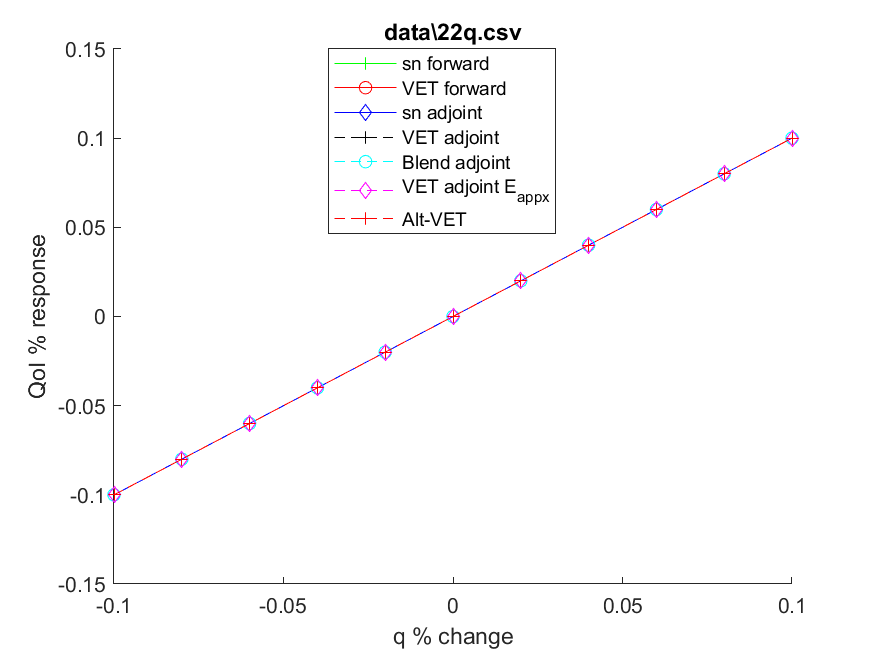
\includegraphics[width=.98\linewidth]{figures2/22qSens.png}
  \label{T1:sfig1}
\end{subfigure}%
\begin{subfigure}{.5\textheight}
  \centering
  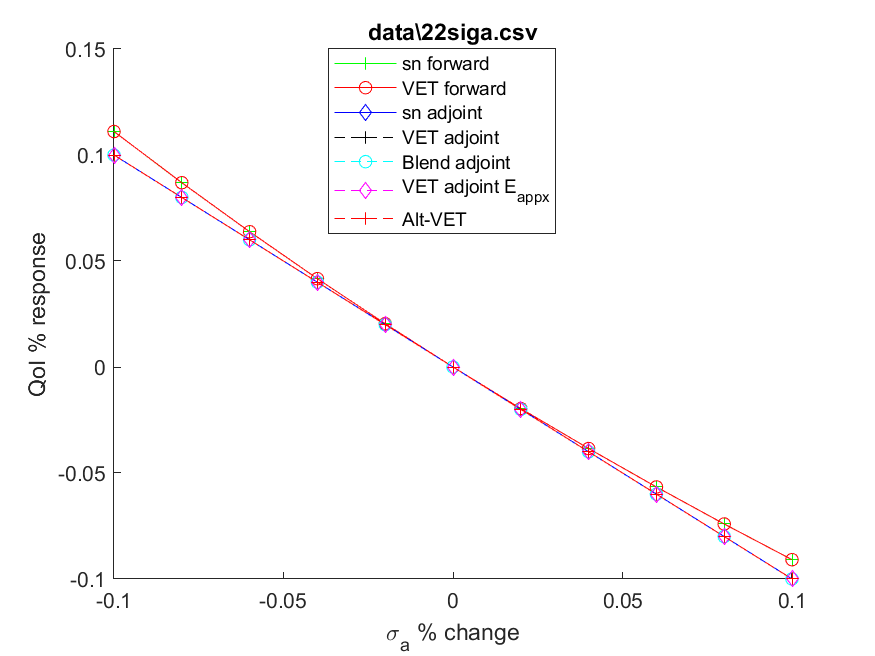
\includegraphics[width=.98\linewidth]{figures2/22sigaSens.png}
  \label{T1:sfig2}
\end{subfigure}
%
\begin{subfigure}{.5\textheight}
  \centering
  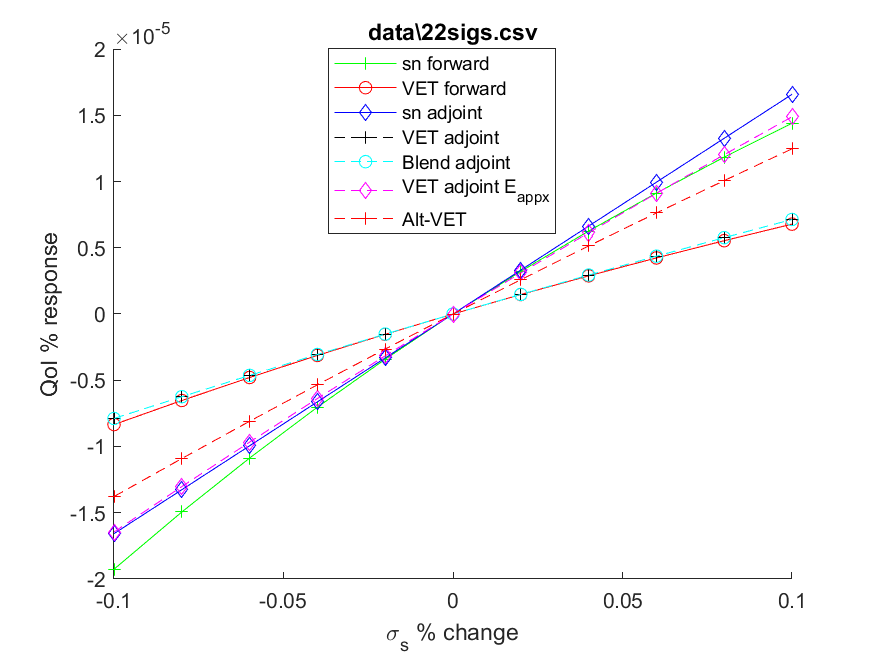
\includegraphics[width=.98\linewidth]{figures2/22sigsSens.png}
  \label{T1:sfig3}
\end{subfigure}%
\begin{subfigure}{.5\textheight}
  \centering
  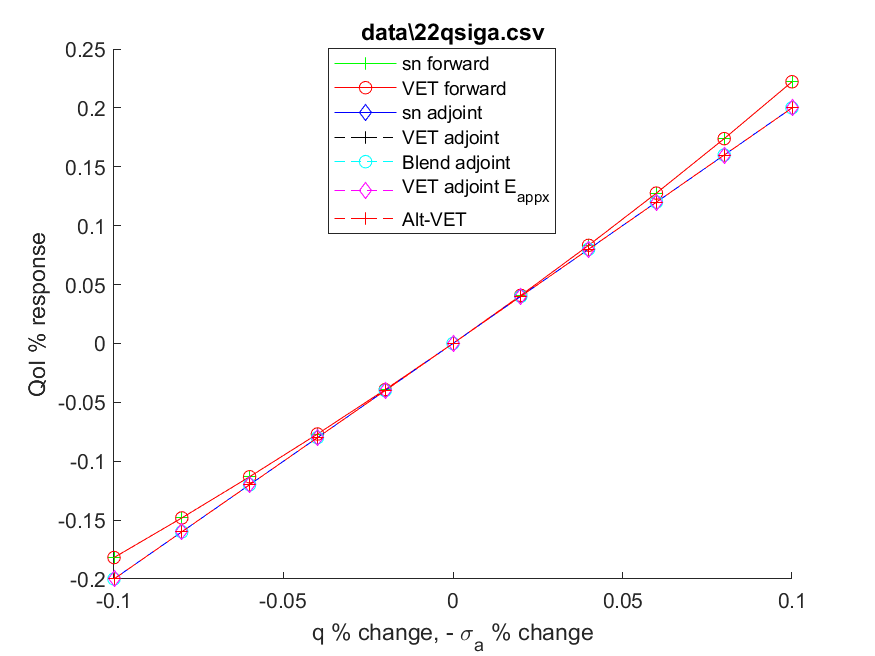
\includegraphics[width=.98\linewidth]{figures2/22qsigaSens.png}
  \label{T1:sfig4}
\end{subfigure}
\end{figure}
\end{flushleft}
\end{frame}

\begin{frame}\frametitle{Homogeneous System, Homogeneous Perturbation}
 \begin{flushleft}
\begin{table}[H]
\label{TableT1}
\centering
  \begin{tabular}{| l | r | r | r | r |}
    \hline
    Method  &  $+10\% q $  & $-10\% \siga $ & $+10\% \sigs $ & $+10\% q,-10\% \siga$ \\ \hline
     SN Fwd 			&0.39998 &0.44419 &5.7577e-05 & 0.88858\\ \hline
     VET Fwd			&0.39998 &0.44428 &2.7131e-05 &0.88868\\ \hline
     SN Adj			&0.39998 &0.39983 &6.6307e-05 &0.79980\\ \hline
     VET Adj 			&0.39998 &0.39988 &2.8534e-05 &0.79986\\ \hline
     Blended 			&0.39998 &0.39988 &2.8534e-05 &0.79986\\ \hline
     VET $\delta \Edd$ 	&0.39998 &0.39983 &5.9537e-05 &0.79981\\ \hline
     VET Alt			& --  & --  &	--		&  --\\ \hline
    \end{tabular}
  \caption{Table of selected results for the homogeneous system under homogeneous perturbations. Values given are absolute $\delta \Edd$. }
\end{table}
\end{flushleft}
\end{frame}


\begin{frame}\frametitle{Homogeneous System, Non-Homogeneous Perturbation}
 \begin{flushleft}

\begin{figure}[H]
\label{Trial1}
\centering
\begin{subfigure}{.5\textheight}
  \centering
  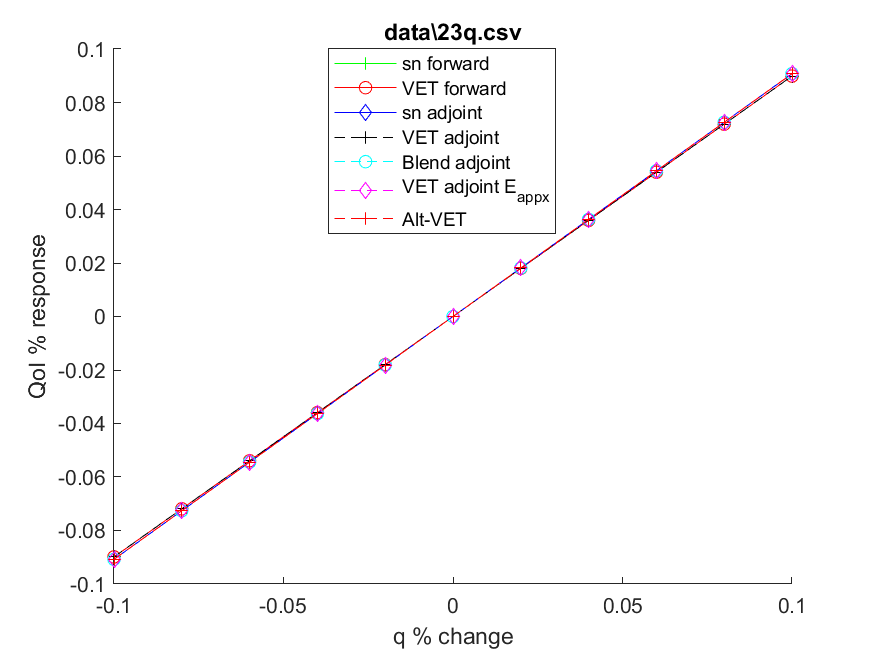
\includegraphics[width=.98\linewidth]{figures2/23qSens.png}
  \label{T1:sfig1}
\end{subfigure}%
\begin{subfigure}{.5\textheight}
  \centering
  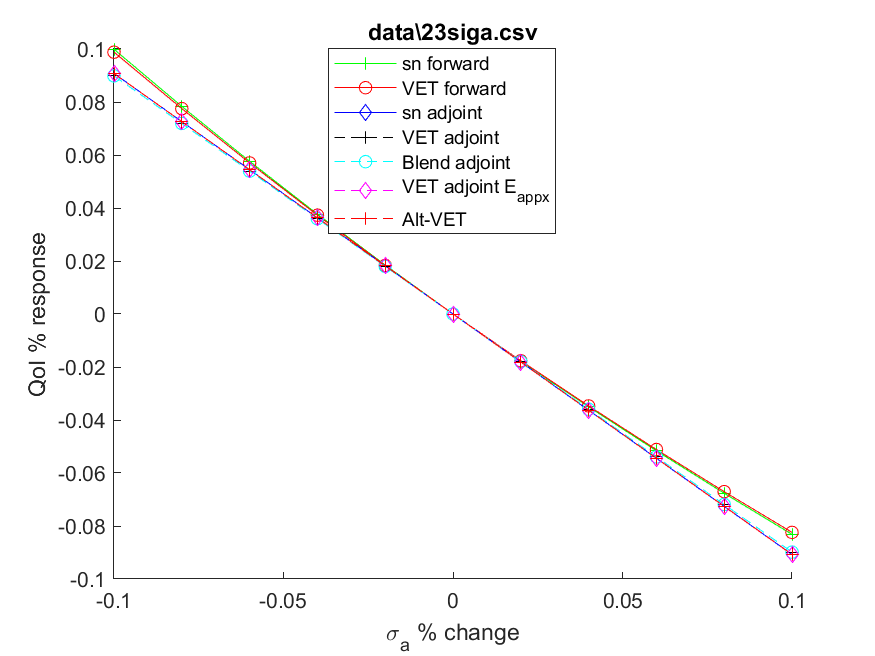
\includegraphics[width=.98\linewidth]{figures2/23sigaSens.png}
  \label{T1:sfig2}
\end{subfigure}
%
\begin{subfigure}{.5\textheight}
  \centering
  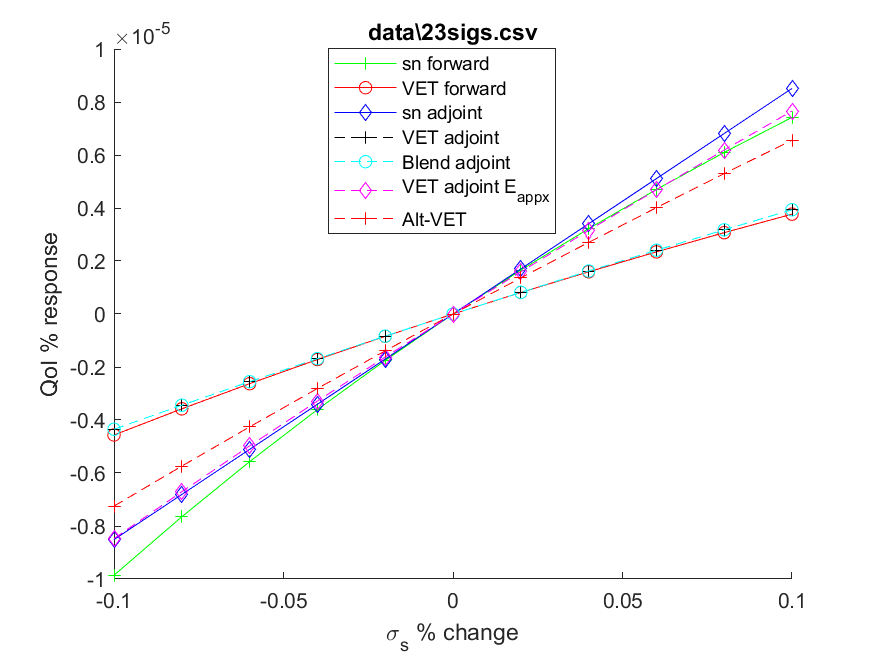
\includegraphics[width=.98\linewidth]{figures2/23sigsSens.png}
  \label{T1:sfig3}
\end{subfigure}%
\begin{subfigure}{.5\textheight}
  \centering
  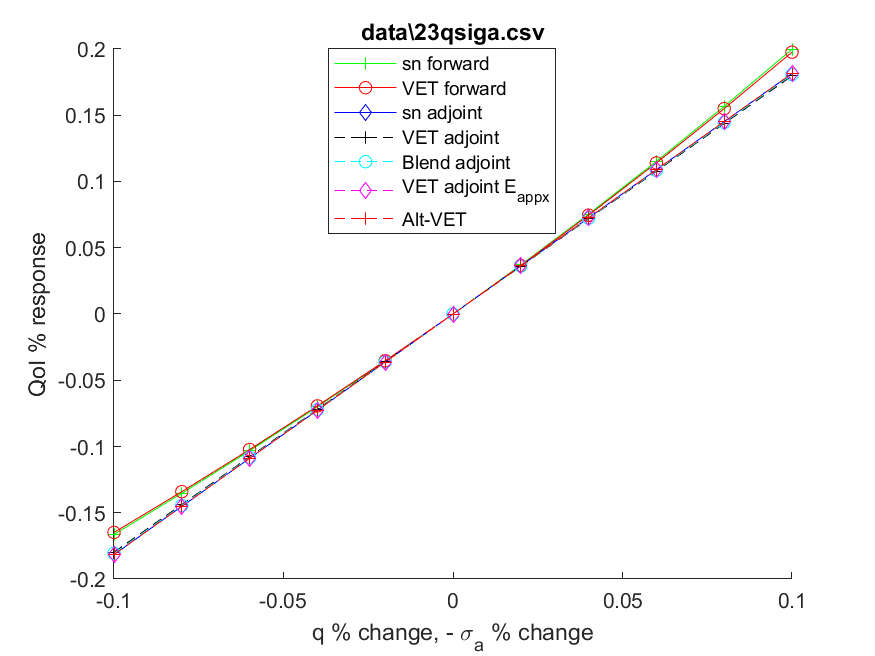
\includegraphics[width=.98\linewidth]{figures2/23qsigaSens.png}
  \label{T1:sfig4}
\end{subfigure}
\end{figure}
\end{flushleft}
\end{frame}

\begin{frame}\frametitle{Homogeneous System, Non-Homogeneous Perturbation}
 \begin{flushleft}
\begin{table}[H]
\centering
  \begin{tabular}{| l | r | r | r | r |}
    \hline
    Method  &  $+10\% q $  & $-10\% \siga $ & $+10\% \sigs $ & $+10\% q,-10\% \siga$ \\ \hline
     SN Fwd 			&0.36309 &0.39952 &2.9680e-05 & 0.79915\\ \hline
     VET Fwd			&0.35947 &0.39517 &1.5072e-05 &0.79040\\ \hline
     SN Adj  			&0.36309 &0.36301 &3.4051e-05 &0.72610\\ \hline
     VET Adj 			&0.35947 &0.35941 &1.5733e-05 &0.71888\\ \hline
     Blended 			&0.36309 &0.35941 &1.5733e-05 &0.72250\\ \hline
     VET $\delta \Edd$ 	&0.36287 &0.36290 &3.0640e-05 &0.72586\\ \hline
     VET Alt			& --  & --  &	--		&  --\\ \hline
    \end{tabular}
  \caption{Table of selected results for the homogeneous system under inhomogeneous perturbations. Values given are absolute $\delta \Edd$. }
\end{table}
\end{flushleft}
\end{frame}


\begin{frame}\frametitle{Shielded Incident Flux}
 \begin{flushleft}

\begin{figure}[H]
\label{Trial1}
\centering
\begin{subfigure}{.5\textheight}
  \centering
  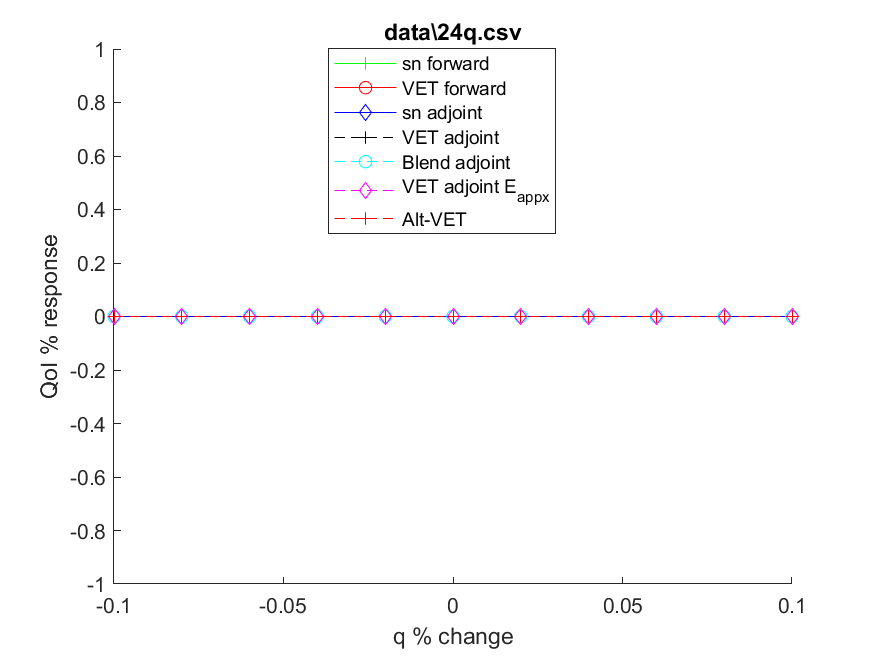
\includegraphics[width=.98\linewidth]{figures2/24qSens.png}
  \label{T1:sfig1}
\end{subfigure}%
\begin{subfigure}{.5\textheight}
  \centering
  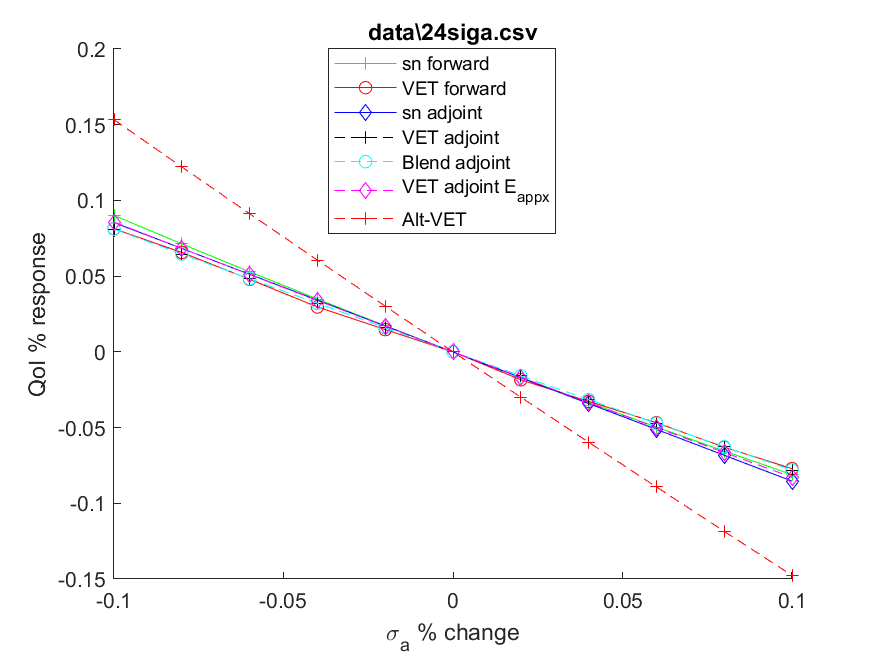
\includegraphics[width=.98\linewidth]{figures2/24sigaSens.png}
  \label{T1:sfig2}
\end{subfigure}
%
\begin{subfigure}{.5\textheight}
  \centering
  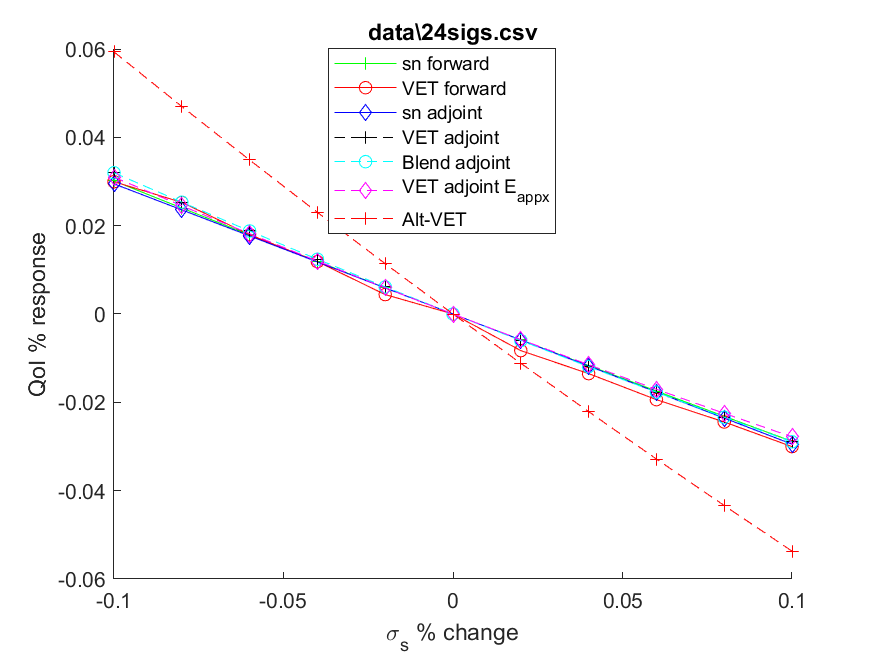
\includegraphics[width=.98\linewidth]{figures2/24sigsSens.png}
  \label{T1:sfig3}
\end{subfigure}%
\begin{subfigure}{.5\textheight}
  \centering
  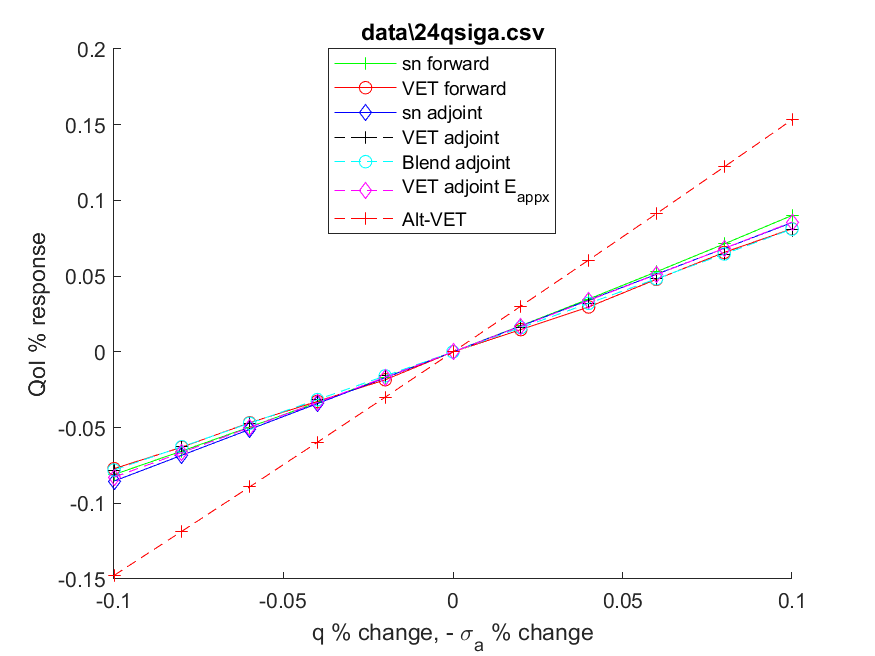
\includegraphics[width=.98\linewidth]{figures2/24qsigaSens.png}
  \label{T1:sfig4}
\end{subfigure}
\end{figure}
\end{flushleft}
\end{frame}

\begin{frame}\frametitle{Homogeneous System, Non-Homogeneous Perturbation}
 \begin{flushleft}
\begin{table}[H]
\centering
  \begin{tabular}{| l | r | r | r | r |}
    \hline
    Method  &  $+10\% \psi^- $  & $-10\% \siga $ & $+10\% \sigs $ & $+10\% \psi^-,-10\% \siga$ \\ \hline
     SN Fwd 			&0.023401 &0.021079 &-0.0067476 & 0.046588\\ \hline
     VET Fwd			&0.023181 &0.019670 &-0.0066481 &0.044818\\ \hline
     SN Adj  			&0.023401 &0.019975 &-0.0068956 &0.043376\\ \hline
     VET Adj 			&0.023181 &0.018981 &-0.0067751 &0.042162\\ \hline
     Blended 			&0.023401 &0.018981 &-0.0067751 &0.042381\\ \hline
     VET $\delta \Edd$ 	&0.023181 &0.020070 &-0.0065156 &0.043251\\ \hline
     VET Alt			&0.023401 &0.035869 &	--		&  --\\ \hline
    \end{tabular}
  \caption{Table of selected results for the shielding system under perturbations. Values given are absolute $\delta \Edd$. }
\end{table}
\end{flushleft}
\end{frame}

%%%%%%%%%%%%%%%%%%%%%%%%%%%%%%%%%%%%%%%%%%%%%%%%%%%%%%%%%%%%%%%%%%%%%%%%%%%%%%%%%%%%%%%%%%%%%%%%%%%%%%%%%%%
%%%%%%%%%%%%%%%%%%%%%%%%%%%%%%%%%%%%%%%%%%%%%%%%%%%%%%%%%%%%%%%%%%%%%%%%%%%%%%%%%%%%%%%%%%%%%%%%%%%%%%%%%%%

%%%%%%%%%%%%%%%%%%%%%%%%%%%%%%%%%%%%%%%%%%%%%%%%%%%%%%%%%%%%%%%%%%%%%%%%%%%%%%%%%%%%%%%%%%%%%%%%%%%%%%%%%%%
\section{Wrap Up}	% define sections here, it is possible to get section slides automatically, but this is not enabled
\subsection{}	% we have to keep these to get the navigation
%%%%%%%%%%%%%%%%%%%%%%%%%%%%%%%%%%%%%%%%%%%%%%%%%%%%%%%%%%%%%%%%%%%%%%%%%%%%%%%%%%%%%%%%%%%%%%%%%%%%%%%%%%%
 %%%%%%%%%%%%%%%%%%%%%%%%%%%%%%%%%%%%%%%%%%%%%%%%%%%%%%%%%%%%%%%%%%%%%%%%%%%%%%%%%%%%%%%%%%%%%%%%%%%%%%%%%%%

\begin{frame}\frametitle{Solver}
\begin{flushleft}
\begin{itemize}
\item (Final remarks, next steps, issues with scattering in 1D, references,)
\end{itemize}
\end{flushleft}
\end{frame}

\end{document}